\documentclass[]{politex}

% ========== Packages ==========
\usepackage[utf8]{inputenc}
\usepackage{amsmath,amsthm,amsfonts,amssymb}
\usepackage{graphicx,cite,enumerate}
\usepackage{subfiles}
\usepackage{caption}
\usepackage{pdfpages}
\usepackage{adjustbox}
\usepackage{wrapfig,lipsum}
\usepackage{verbatim}
\usepackage{listings}
\usepackage{array}

% ========== Language options ==========
\usepackage[brazil]{babel}

% ========== ABNT (requer ABNTeX 2) ==========
%	http://www.ctan.org/tex-archive/macros/latex/contrib/abntex2
\usepackage[num]{abntex2cite}

% ========== Lorem ipsum ==========
\usepackage{blindtext}

% ========== Opções do documento ==========
% Título
\titulo{Desenvolvimento de Equipamentos para Hospital Universitário da USP}

% Autor
\autor{Thomaz Akira Furukawa}

% Orientador / Coorientador
\orientador{Leopoldo Rideki Yoshioka}
\coorientador{Oswaldo Horikawa}

% Tipo de documento
\tcc{}
%\dissertacao{Engenharia Elétrica}
%\teseDOC{Engenharia Elétrica}
%\teseLD
%\memorialLD

% Departamento e área de concentração
\departamento{Engenharia de Sistemas Eletrônicos}
\areaConcentracao{Engenharia Mecatrônica}

% Local
\local{São Paulo}

% Ano
\data{2022}

\begin{document}
% ========== Capa e folhas de rosto ==========
\capa
\falsafolhaderosto
\folhaderosto

%========== Folha de assinaturas (opcional) ==========
%\begin{folhadeaprovacao}
	\assinatura{Prof. Dr. Leopoldo Rideki Yoshioka}
	\assinatura{Prof. Dr. Oswaldo Horikawa}
%	\assinatura{Prof.\ Y}
%	\assinatura{Prof.\ Z}
%\end{folhadeaprovacao}


% ========== Dedicatória (opcional) ==========
\dedicatoria{Dedico esse trabalho aos atuais e futuros integrantes da ZIMA - Soluções Medico Hospitalares}

% ========== Agradecimentos ==========
\begin{agradecimentos}

Primeiramente, à minha família, que me forneceram inspiração, suporte emocional e financeiro para que eu chegasse até a universidade.

Ao meus professores orientadores, Leopoldo Yoshioka, pela a oportunidade de participar do grupo , fazer a manutenção do projeto e sempre dar suporte, tanto em ajuda, quanto em ensinamentos através de boas conversas e alguma risadas. Ao Professor Oswaldo Horikawa, que foi um forte auxílio técnico no desenvolvimento dos projetos e me inspirou a ser um engenheiro melhor.

Aos coordenadores de área e antigos membros, Vanderson Santos, Lucas Boccia, Lucas Grob, Wu Kam Long, Pedro Croso, Caio Oliveria, Lucas Junji e Joao Magano que sem essa equipe nada do que será apresentado seria possível.


\end{agradecimentos}

% ========== Epígrafe (opcional) ==========
\epigrafe{%
	\emph{``Para ganhar, tem que jogar bem e dar sorte.''}
	\begin{flushright}
		- Josué Ramalho da Silva
	\end{flushright}
}

% ========== Resumo ==========
\begin{resumo}
Desde 2020, a Escola Politécnica e Hospital Universitário da USP colaboram juntos para o desenvolvimento de soluções tecnológicas na área da saúde. O trabalho de incentivo a inovação foi o responsável pelo projeto Robô Hospitalar, robô autônomo para entregas de exames laboratorias, que chamou atenção dos colaboradores do Hospital para as oportunidades de inserir a tecnologia para inovar na saúde. Com o desenvolvimento do projeto e a entrega de resutados concretos, novas oportunidades surgiram, sendo duas delas sementes de dois novos projetos: o Dispensador de Remédios da Farmácia do HU e o aparelho de reabilitação Ciclo Ergômetro. Com a aproximação da Escola Politécnica e o Hospital Universitário da USP o incentivo a inovação se deu de diversas maneiras, não se limitando a entrega de projetos mas também a criação de grupos focados em inovação na saúde.
%
\\[3\baselineskip]
%
\textbf{Palavras-Chave} -- Automação, Algoritmos de Controle, Programação de Embarcados, Robótica, Saúde, Eletromédicos, Hospitalar, Inovação.
\end{resumo}

\begin{comment}

% ========== Abstract ==========
\begin{abstract}
Abstract...
%
\\[3\baselineskip]
%
\textbf{Keywords} -- Word, Word, Word, Word, Word.
\end{abstract}
\end{comment}
% ========== Listas (opcional) ==========
\listadefiguras

% ========== Sumário ==========
\sumario

% ========== Elementos textuais ==========

% ========== Parte 1: Introdução ==========
\part{Introdução}
\subfile{chapters/introducao} % em qual contexto foi possivel realizar a construção das maquinas e a criação da zima

\subfile{chapters/objetivo} % objetivo golgi ciclo robo e zima

\subfile{chapters/motivacao} % motivação

\subfile{chapters/metodologia} % como foi a concepção e fabricação

\subfile{chapters/arquitetura_do_projeto} % como a equipe se organizou e qual é a arquitetura de cada um

% ========== Parte 2: Golgi Bot ==========
\part{Golgi Bot} 
O diagrama abaixo divide o equipamento em subsistemas, cada um com determinada função e aplicações mecânicas, eletrônicas ou computacionais.

\begin{figure}[h]
	\centering
		\caption{Diagrama Projeto Golgi Bot}
		\centering % para centralizarmos a figura
		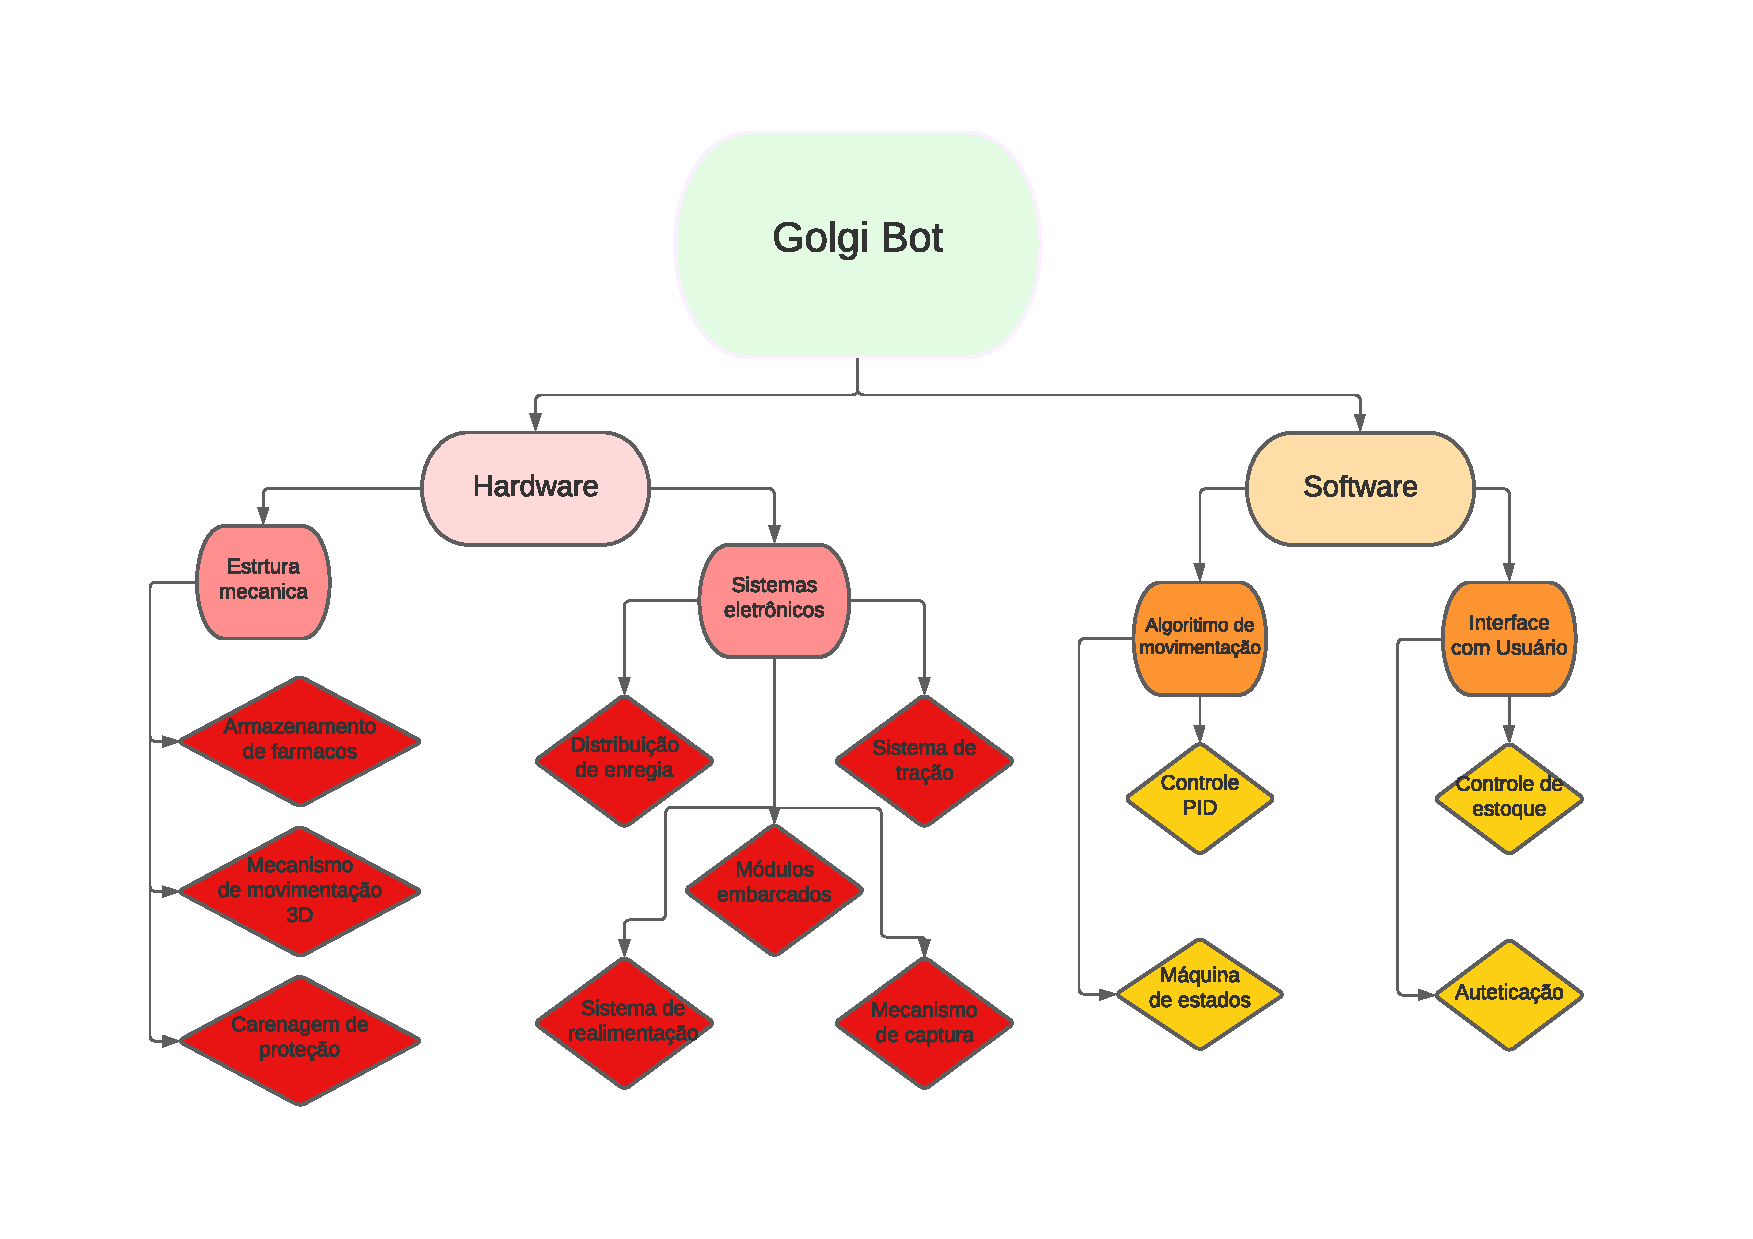
\includegraphics[width=17cm]{docs/golgi_bot_general_diagram.pdf}
		\caption*{Fonte: Autor}
		\label{figura:Diagrama Projeto Golgi Bot}
	\end{figure}
	
\subfile{chapters/hardware_golgi}

\subfile{chapters/software_golgi}

% ========== Parte 3: Ciclo Êrgometro  ==========
\part{Ciclo Êrgometro} 
O diagrama abaixo divide o equipamento em subsistemas, cada um com determinada função e aplicações mecânicas, eletrônicas ou computacionais.

\begin{figure}[h]
	\centering
		\caption{Diagrama Projeto Ciclo}
		\centering % para centralizarmos a figura
		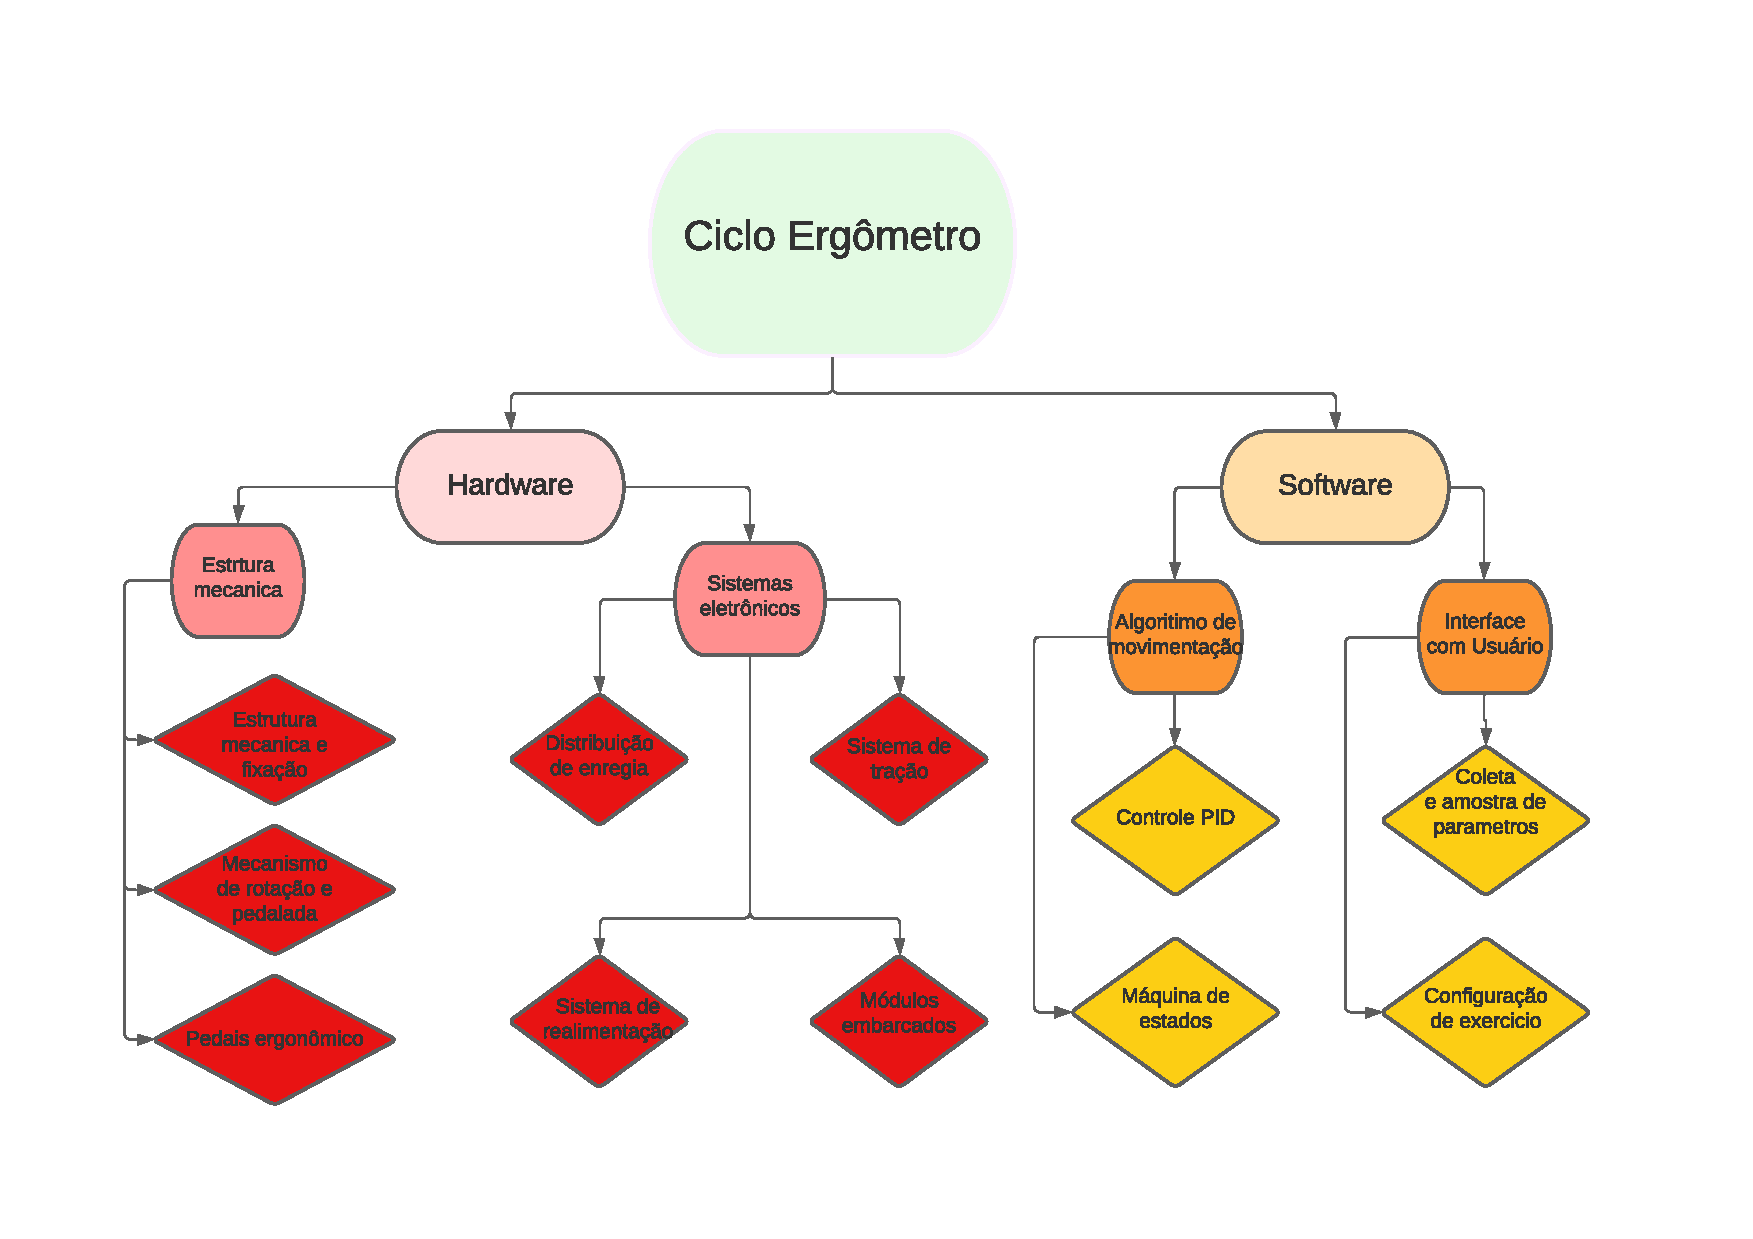
\includegraphics[width=17cm]{images/Diagrama ciclo.pdf}
		\caption*{Fonte: Autor}
		\label{figura:Diagrama Projeto Ciclo}
	\end{figure}
\subfile{chapters/hardware_ciclo}

\subfile{chapters/software_ciclo}

% ========== Parte 4: Hema bot ==========
\part{Hema Bot} 

\subfile{chapters/v3}

% ========== Parte 5: Zima ==========
\part{ZIMA} 


\subfile{chapters/estrutura_zima}

\begin{comment} % se sobrar tempo comentar


\end{comment}

% ========== Parte 4: Software ==========
\part{Resultados}

No projeto Golgi Bot, Automação da Farmácia do HU, foram frabricados o primeiro mini prototipo funcional o qual foi capaz de capturar remedios e se movimentar como esperado. Os sistemas eletronicos e modulos embarcados foram fabricados e atualmente se encontramos na versão em escala real que a movimentação esta sendo testada para iniciar os teste de captura.Além disso, foram realizadas diversas reuniões com os coolaboradores do HU em função do software que já possui versão funcional mas segue em melhorias

\begin{figure}[h]
\centering
    \begin{minipage}{0.5\textwidth}
       \centering
        \caption{Modulo movimentação Golgi}
        \centering % para centralizarmos a figura
        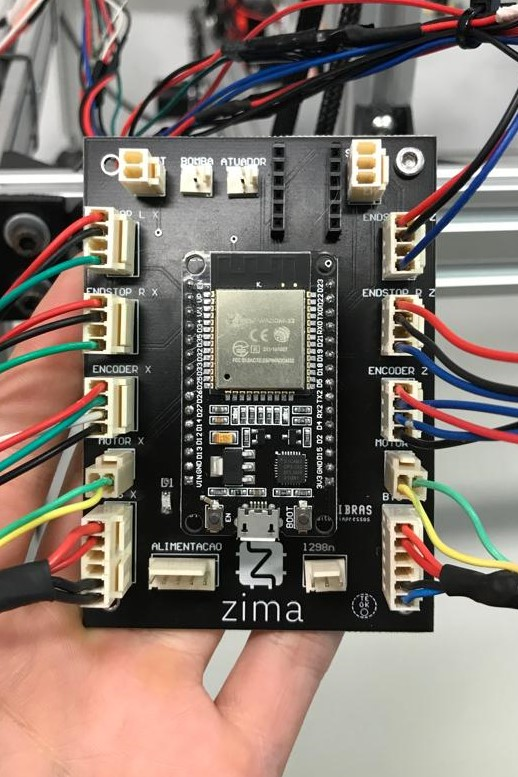
\includegraphics[width=4cm]{images/modulo_golgi.jpeg}
        \caption*{Fonte: Autor}
        \label{figura: Modulo movimentação Golgi}
        
    \end{minipage}\hfill
    \begin{minipage}{0.5\textwidth}
        \centering
        \caption{Reunião Farmácia (HU)}
        \centering % para centralizarmos a figura
        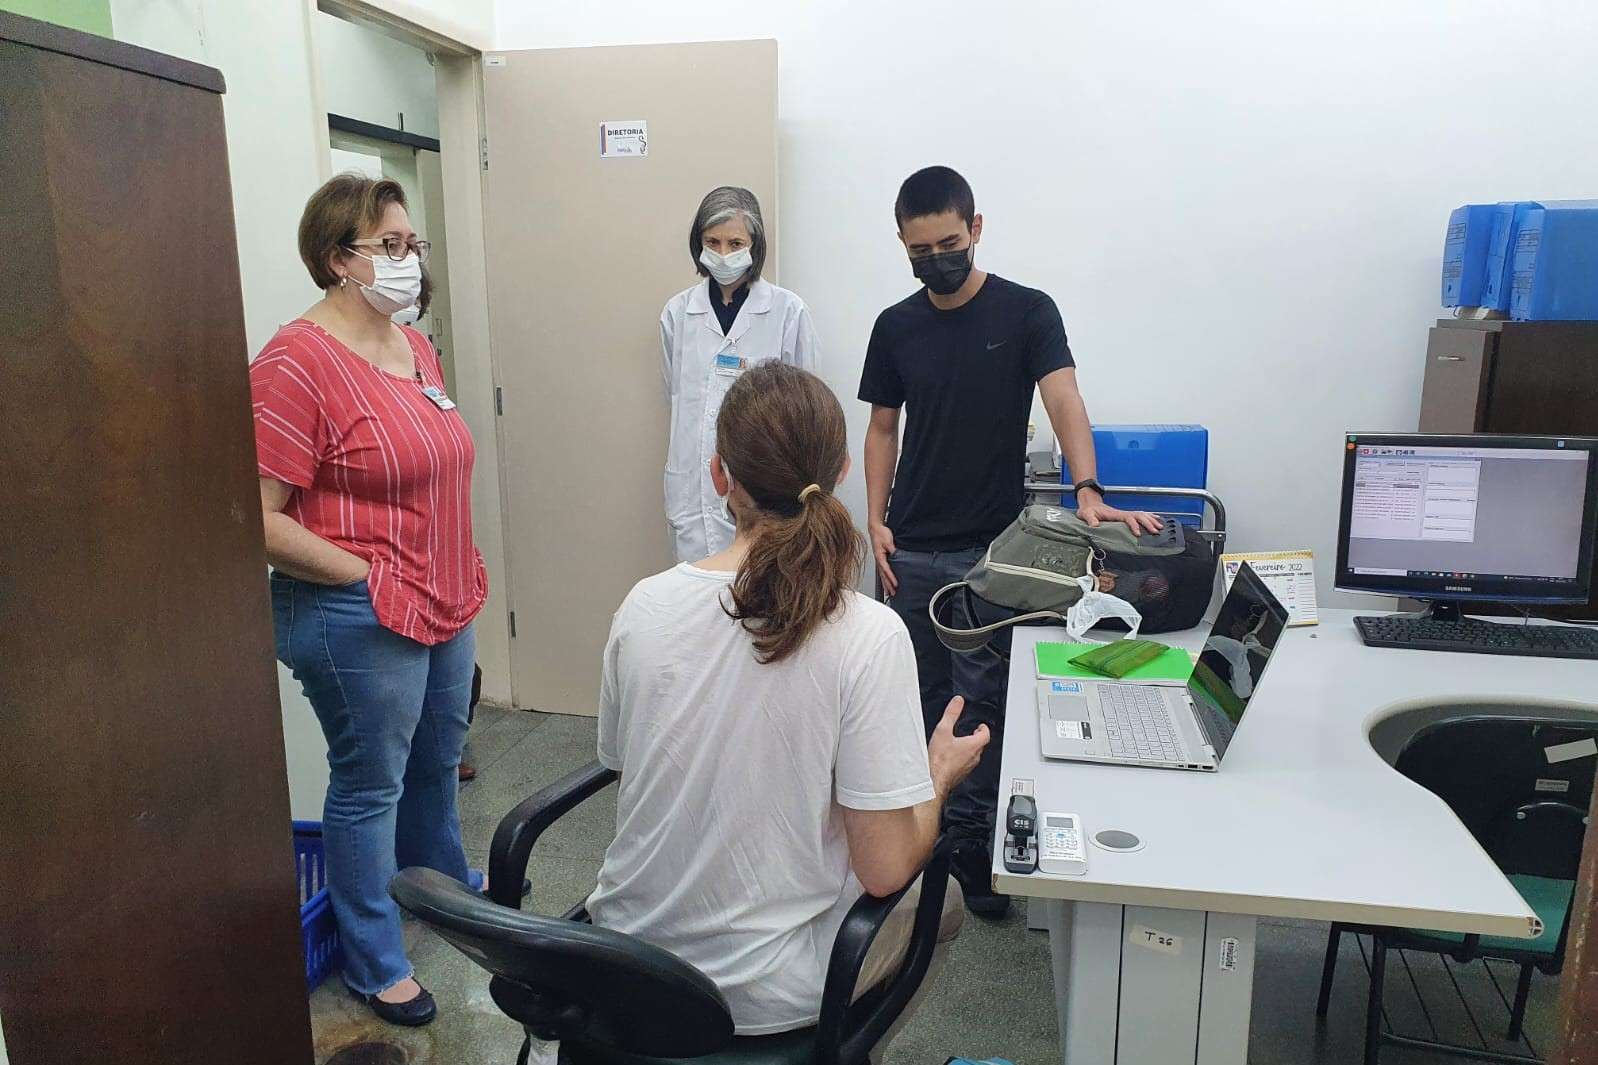
\includegraphics[width=9cm]{images/reuni_golgi.jpg}
        \caption*{Fonte: Autor}
        \label{figura: Reunião Farmácia (HU)}
    \end{minipage}\hfill
\end{figure}
\begin{figure}[h]
\centering
    \begin{minipage}{0.5\textwidth}
       \centering
        \caption{Golgi Bot miniatura}
        \centering % para centralizarmos a figura
        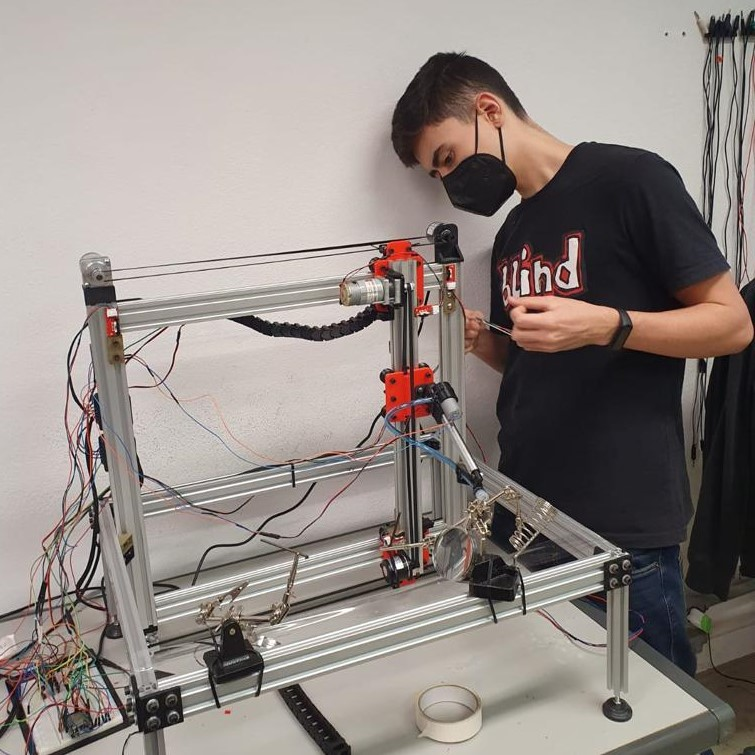
\includegraphics[width=8cm]{images/minigolgi.jpeg}
        \caption*{Fonte: Autor}
        \label{figura: Golgi Bot miniatura}
        
    \end{minipage}\hfill
    \begin{minipage}{0.5\textwidth}
        \centering
        \caption{Golgi Bot tamanho Real}
        \centering % para centralizarmos a figura
        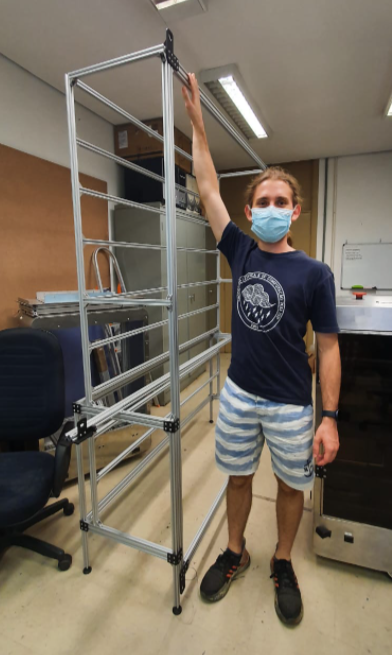
\includegraphics[width=5cm]{images/gigagolgi.png}
        \caption*{Fonte: Autor}
        \label{figura: Golgi Bot tamanho Real}
    \end{minipage}\hfill
\end{figure}

Para o ciclo ergometro foi frabricado toda primeira versão com o modo manual e automático. O equipamento foi completamente montado e testado com mais de 20 voluntários da escola politécnica. Os resultados dos testes comprovaram a ergonomia do equipamento mas ressaltaram pontos que estão sendo corrigidos na segunda versão do cicloergometro. Para garantir o bom andamento do projeto foram feitos acompanhamentos quinzenais com a Dra Alexandra Siqueira e Prof. Oswaldo Horikawa.

\begin{figure}[h]
\centering
    \begin{minipage}{0.5\textwidth}
       \centering
        \caption{Teste Ciclo Ergômetro}
        \centering % para centralizarmos a figura
        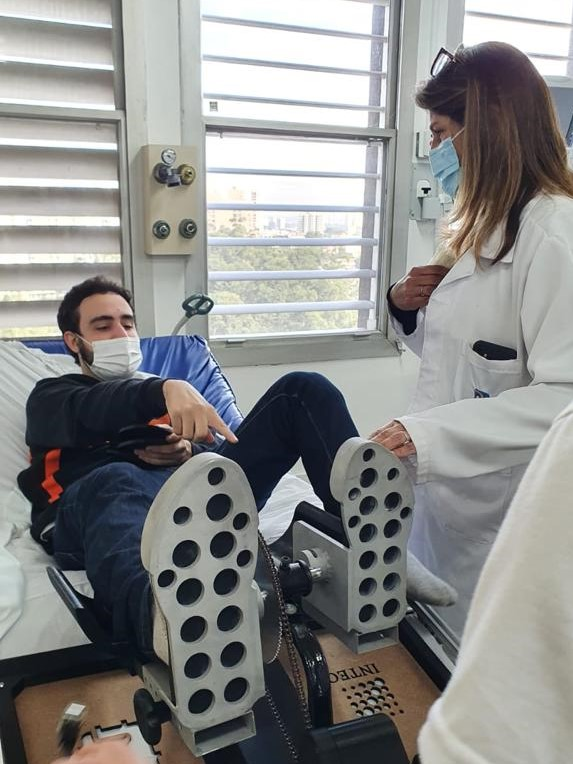
\includegraphics[width=7cm]{images/teste_ciclo.jpeg}
        \caption*{Fonte: Autor}
        \label{figura: Teste Ciclo Ergômetro}
        
    \end{minipage}\hfill
    \begin{minipage}{0.5\textwidth}
        \centering
        \caption{Reunião UTI Adulto}
        \centering % para centralizarmos a figura
        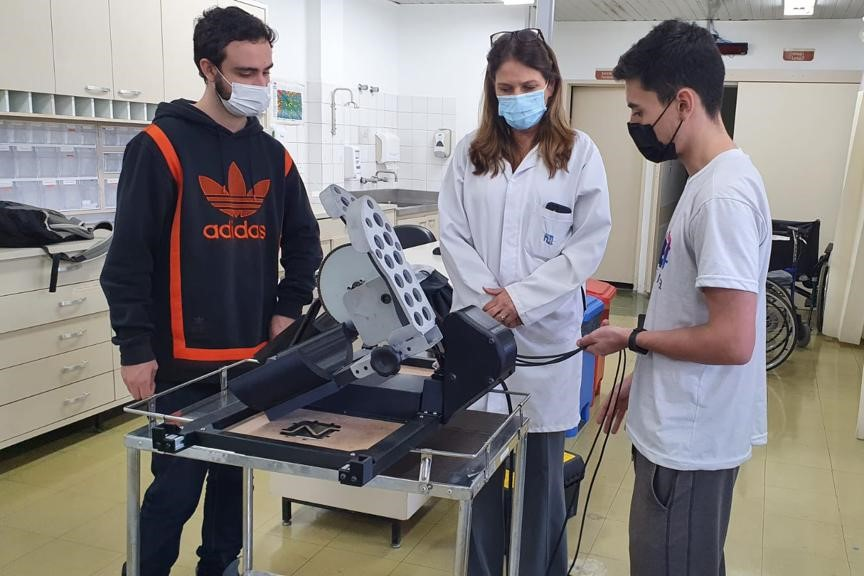
\includegraphics[width=9cm]{images/reuni_ciclo.jpeg}
        \caption*{Fonte: Autor}
        \label{figura: Reunião UTI Adulto}
    \end{minipage}\hfill
\end{figure}


A 3ª versão do robô hospitalar Hema bot, foi concepcionada no CAD e fabricada com PLA no próprio laboratorio. Para isso foi realizado a compra de uma impressora 3D de 30x30x40cm de volume útil. Além disso foi feito a soldagem da nova placa embarcada e realizado os testes de suas funcionalidades.

\begin{figure}[h]
\centering
    \begin{minipage}{0.5\textwidth}
       \centering
        \caption{Fabricação Hema Bot}
        \centering % para centralizarmos a figura
        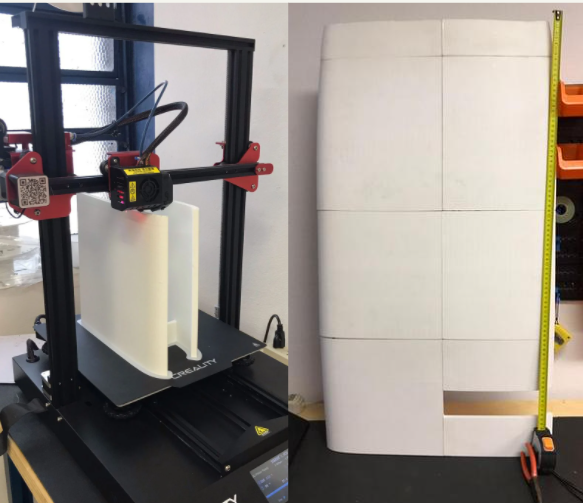
\includegraphics[width=9cm]{images/fabrica_hema.png}
        \caption*{Fonte: Autor}
        \label{figura: Fabricação Hema Bot}
        
    \end{minipage}\hfill
    \begin{minipage}{0.5\textwidth}
        \centering
        \caption{Hema Bot Real}
        \centering % para centralizarmos a figura
        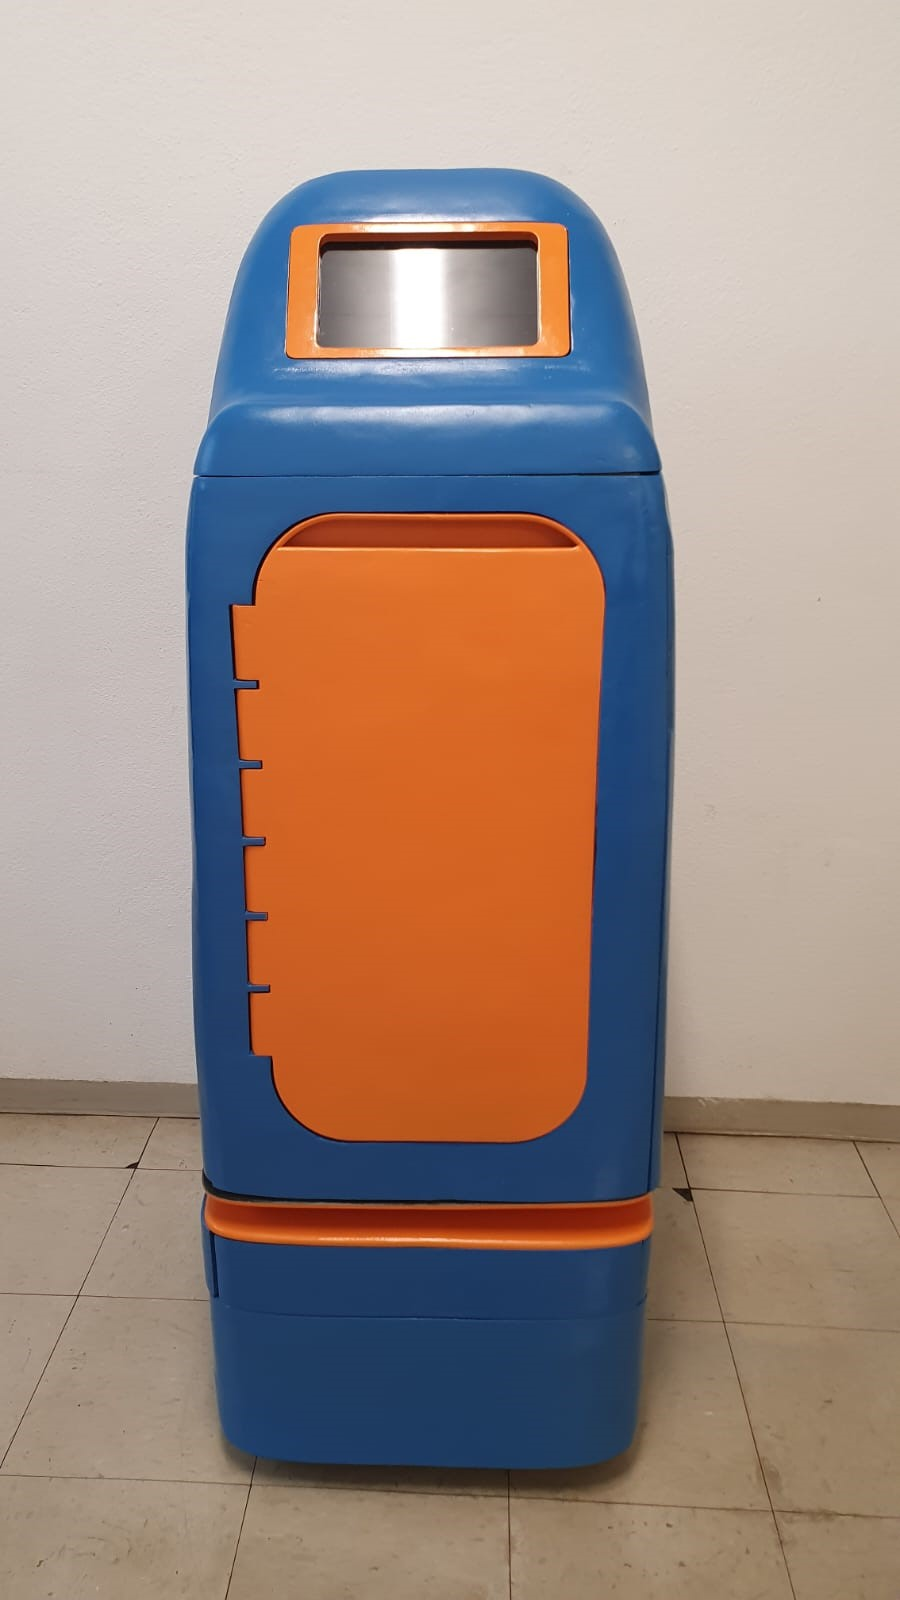
\includegraphics[width=4cm]{images/hemabotreal.jpeg}
        \caption*{Fonte: Autor}
        \label{figura: Hema Bot Real}
    \end{minipage}\hfill
\end{figure}

Já em termos de grupo de extesão, o grupo cresceu para 25 membros ativos e se inseriu na comunidade usp atraves de diversas apariçoes para os novos ingressantes como na semana de extesão, PET mecatrônica e semana de recepção. Foi realizada toda estruturação de cargos assim como um processo seletivo para os futuros ingressantes.Além disso, outros 3 novos projetos foram adicionados ao Leque do grupo, um andadaro, um ciclo ergometro de membro superior e um dispensador de remédios controlados.O ultimo e mais marcante acontecimento foi a oportunidade do grupo de expor todos os projetos no Hospital Universitário da USP, neste evento os todos coolaboradores do HU tiveram contato direto com os projetos e suas motivações.

\begin{figure}[h]
\centering
    \caption{Evento HU 20/04/2022}
    \begin{minipage}{0.5\textwidth}
       \centering
        
        \centering % para centralizarmos a figura
        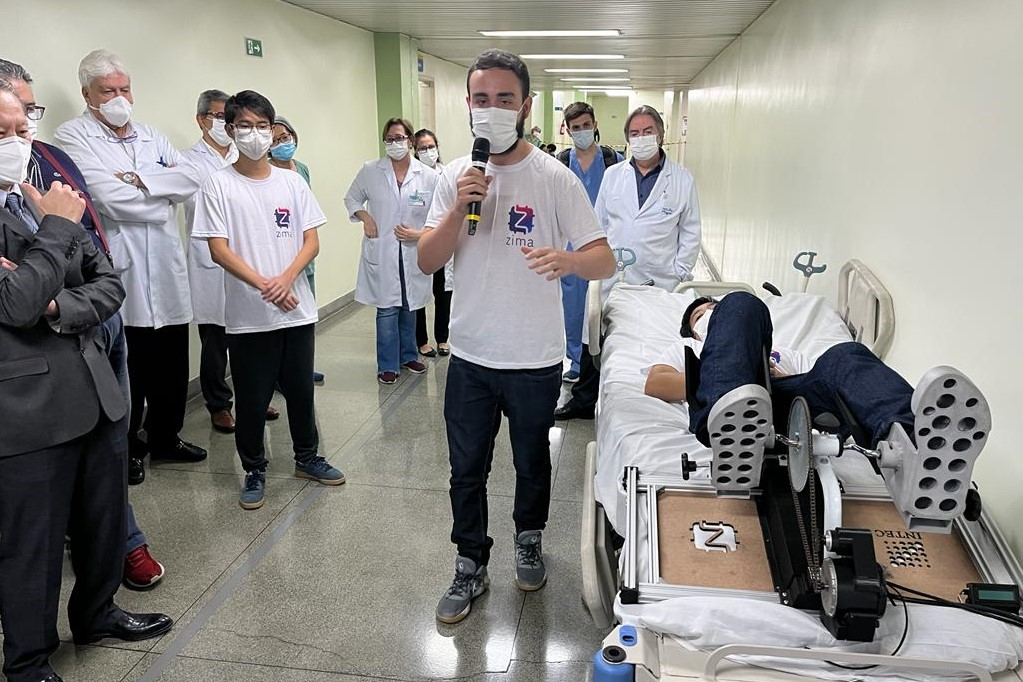
\includegraphics[width=7cm]{images/evento_hu.jpg}
        
        \label{figura: Apresentação HU}
        
    \end{minipage}\hfill
    \begin{minipage}{0.5\textwidth}
        \centering
        \centering % para centralizarmos a figura
        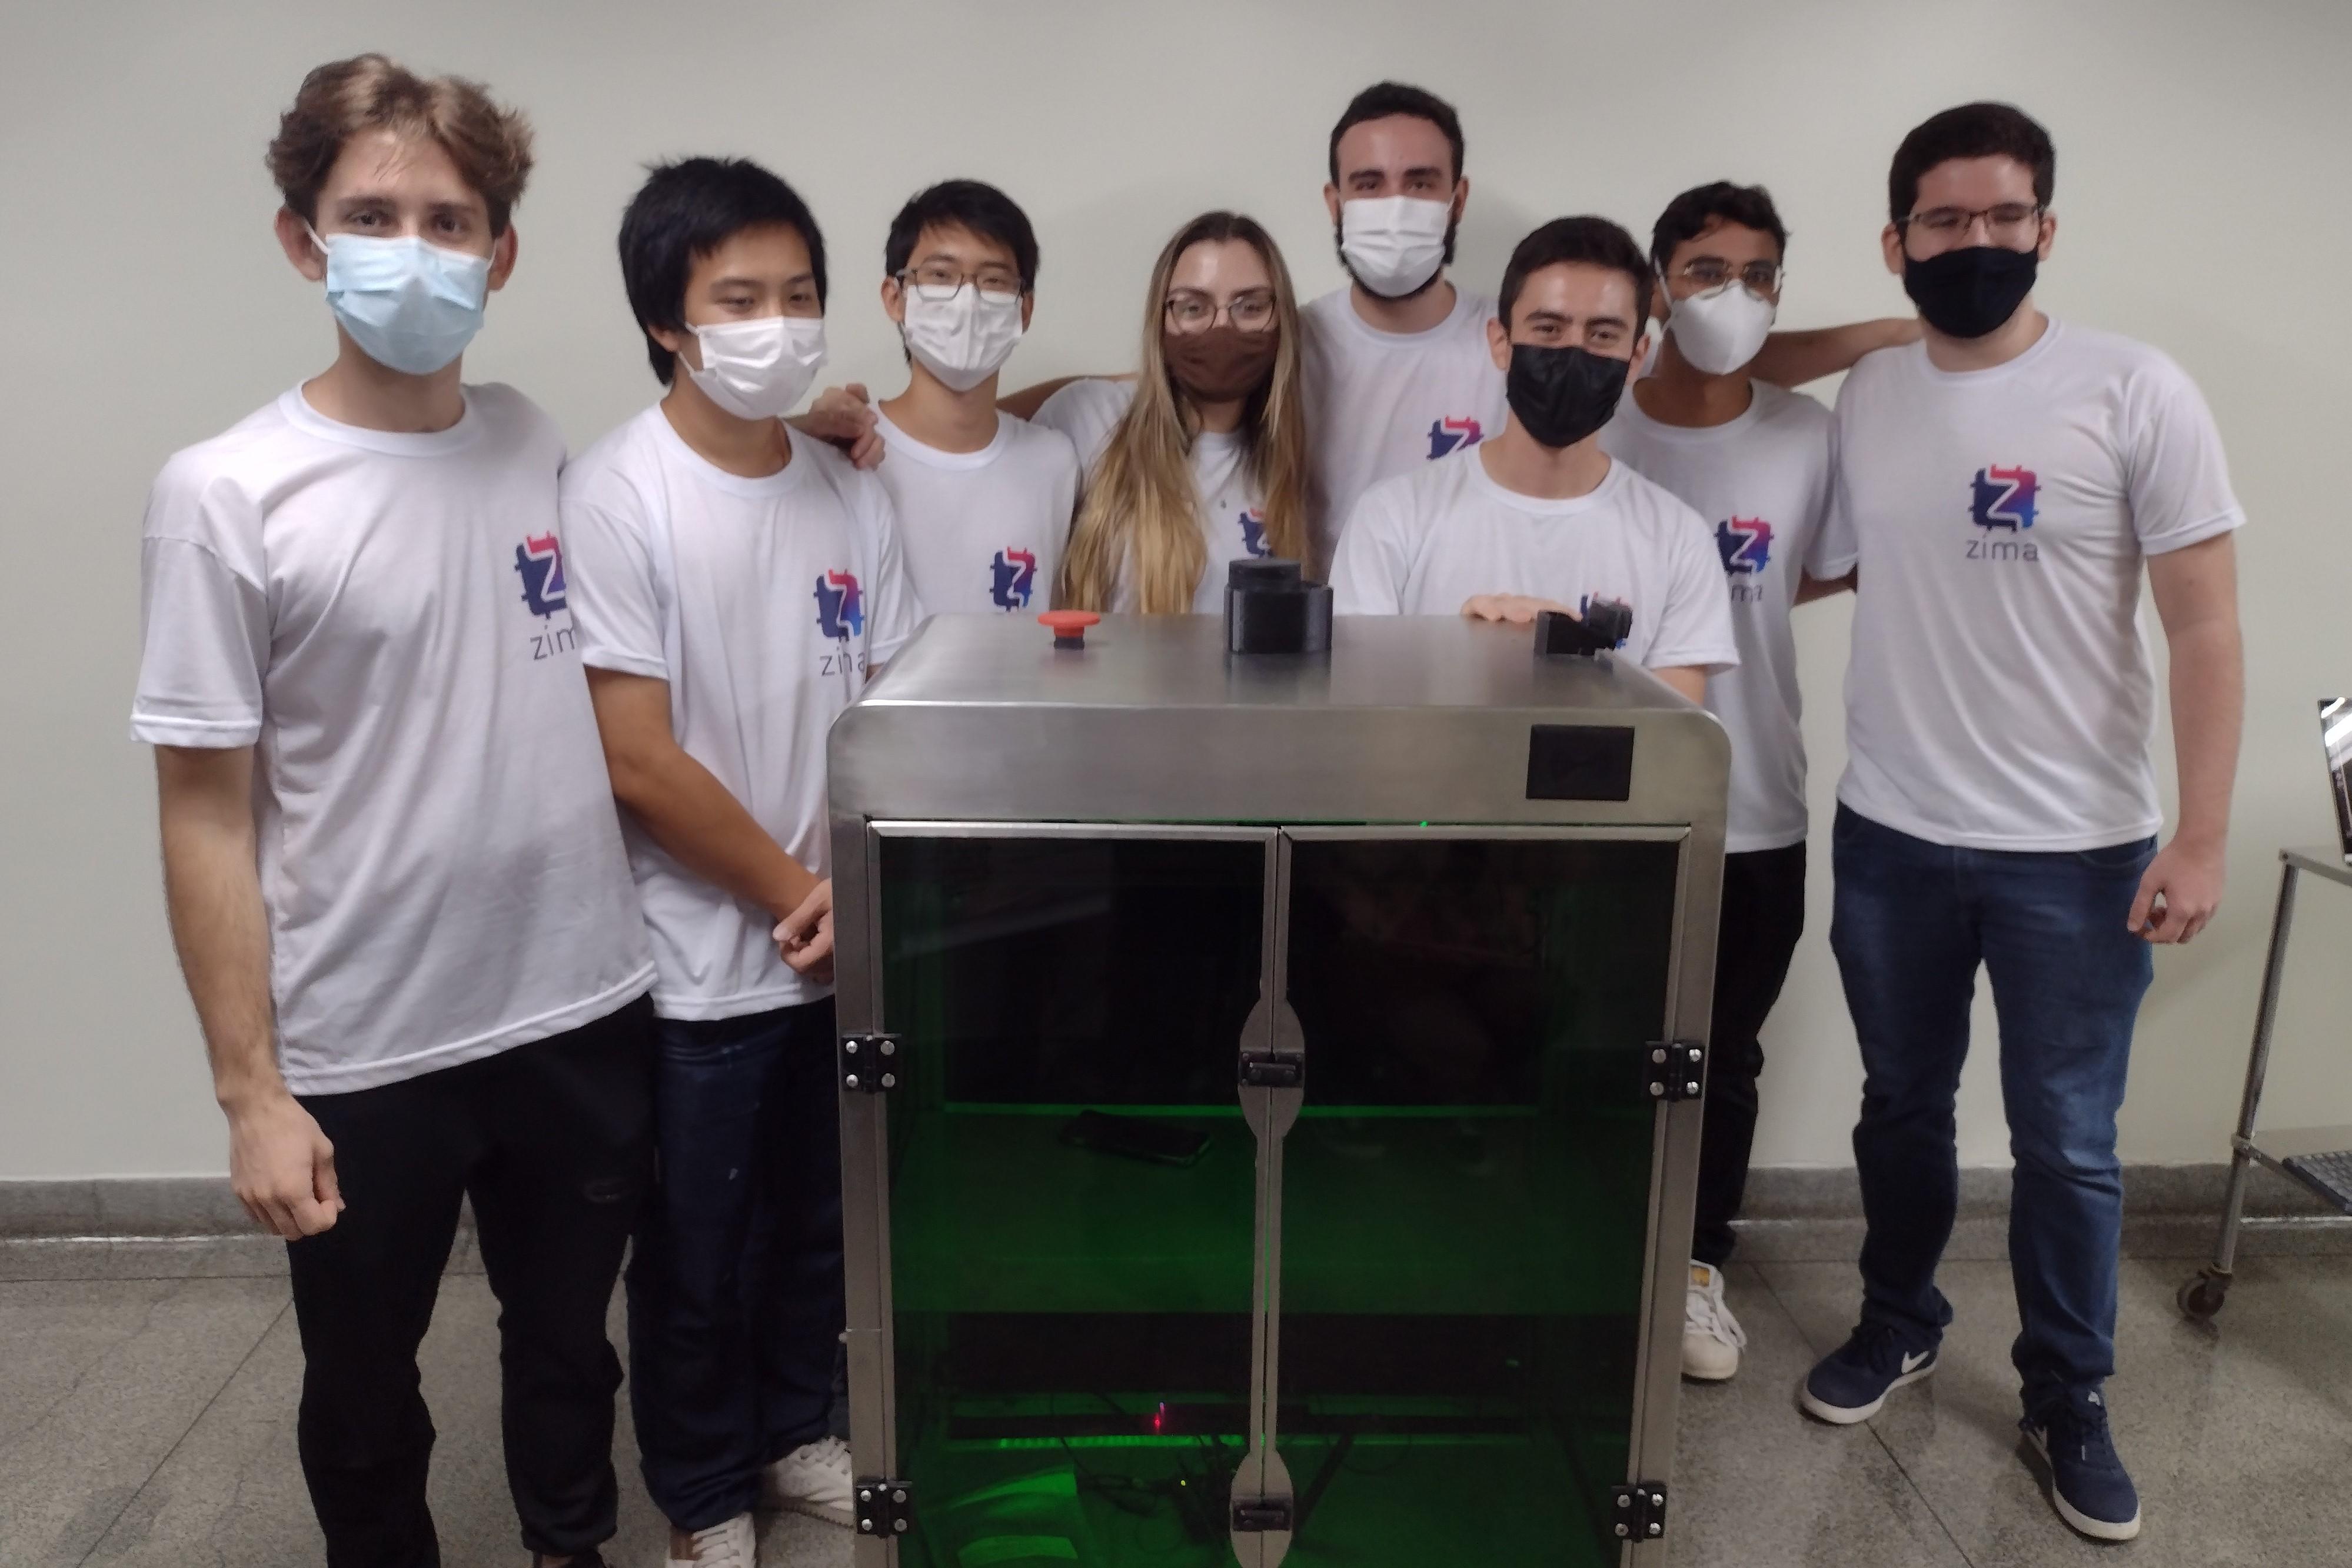
\includegraphics[width=7cm]{images/evento_hu2.jpg}
        \label{figura: Equipe Evento HU}
    \end{minipage}\hfill
    \caption*{Fonte: Autor}
\end{figure}

% ========== TITULOS DO SUMÁRIOS ==========
%\blinddocument
% =========================================

% ========== Referências ==========
% --- ABNT (requer ABNTeX 2) ---
%	http://www.ctan.org/tex-archive/macros/latex/contrib/abntex2
\bibliographystyle{abntex2-num}
\bibliography{bibliography}




\end{document}